\documentclass[11pt]{iopart}
\usepackage{graphics}
\usepackage{epstopdf}
\usepackage{amssymb}
\usepackage{amsfonts}
\usepackage{bbm}
\usepackage{subfigure}
\usepackage{appendix}
\usepackage{pseudocode}
\usepackage{tikz}
\usepackage{pgffor}
\usetikzlibrary{shapes}
\usetikzlibrary{arrows}
\usetikzlibrary{trees}
\usetikzlibrary{patterns}

\begin{document}

\title{A Parallel Multigrid Preconditioner for the Simulation of Large Fracture Networks}

\author{Rahul S. Sampath, Pallab Barai and Phani K.V.V. Nukala}
\address{Computer Science and Mathematics Division, 
Oak Ridge National Laboratory, Oak Ridge, TN 37831-6164, USA}

\begin{abstract}
Computational modeling of fracture in disordered materials using discrete 
lattice models requires the solution of a linear system of equations every time a new lattice 
bond is broken. Solving these linear systems of equations successively is the most expensive
 part of fracture simulations using large three-dimensional networks. In this paper, we present a 
 parallel multigrid preconditioned conjugate gradient algorithm to solve these
 linear systems. Numerical experiments demonstate that this algorithm performs significantly
 better than the algorithms previously used to solve this problem.
\end{abstract}

\section{Introduction}
\label{sec:intro}
Progressive damage evolution leading to failure of disordered
quasi-brittle materials has been studied extensively using various types of discrete lattice models
\cite{hansen00, advphys}. 
In these discrete lattice models, damage is accumulated progressively by breaking one bond at a time until the 
lattice system falls apart. Algebraically, the process of simulating fracture using these models 
is equivalent to solving a new set of linear equations 
\begin{equation}
\label{eqn:intro1}
{\bf A}_n  {\bf v}_n = {\bf f}_n, ~~~~~ n = 0,1,2,\ldots
\end{equation}
every time a new lattice bond is broken. In this paper, we restrict our attention to the 
cubic lattice system with random fuse model \cite{deArcangelis85}. For this system, 
${\bf A}_n$ represents the lattice conductance matrix, ${\bf f}_n$ is the applied nodal current
 and ${\bf v}_n$ is the nodal potential. Equation \ref{eqn:intro1} is solved successively until the matrix 
${\bf A}_n$ becomes singular (this is when the lattice separates into two pieces). Solving these
equations is the most expensive part of a fracture simulation. 

Large scale numerical simulation of these discrete lattice networks
has been limited due to several reasons: (1) The number of broken bonds at failure, $n_f$, increases with system size\footnote{A cubic 
lattice system of size $L$ has $L$ bonds in each direction.} $L$ as
$n_f \sim O(L^{1.8})$ in 2D and $n_f \sim O(L^{2.7})$ in 3D. So, the number of times
Eq. \ref{eqn:intro1} has to be solved increases with increasing lattice system size, $L$.
(2) Although direct solvers combined with low-rank updating schemes \cite{nukalajpamg1} are efficient 
for simulating fracture networks in 2D, they are not suitable for simulating large 3D networks \cite{nukala07}. Moreover, 
parallelization is essential to simulate large 3D networks and iterative solvers are known to have better parallel scalability
compared to direct solvers. Consequently, parallel iterative solvers are in common use 
for simulating large 3D networks. (3) The convergence 
rate of the standard iterative solvers deteriorates with increasing condition number, 
and for the conductivity matrices encountered in fuse lattice problems, the condition number increases with system size 
$L$. In addition, the condition number increases with the number of broken bonds for a fixed system size $L$ 
\cite{nukala07, nukalajpamg2}. This last property causes the {\it{critical slow down}} associated with the iterative solvers close
to the macroscopic fracture. That is, as the lattice system gets closer
to macroscopic fracture, the number of iterations required to attain a
fixed accuracy increases significantly. This becomes particularly significant for large lattices. (4) Although the
 performance of iterative solvers can be significantly improved with the use of good preconditioners, to our 
 knowledge, the best preconditioner used until now to simulate large 3D 
fracture networks in parallel has been the block-Jacobi
preconditioner in which the incomplete LU factorization ( ILU(0) ) \cite{saad03} is applied on each block \cite{nukala07}. Using this preconditioner with
the conjugate gradient (CG) algorithm, simulations of cubic lattice systems of sizes up to $L = 128$ were done in Ref. \cite{nukala07}. 
However, since the blocks are not shared by multiple CPUs, the number of 
 blocks increases as the number of CPUs increases and this leads to a deterioration in the performance of the preconditioner \cite{saad03}. 
 Also, to use this preconditioner we must recompute the ILU factors each time a bond is broken, which
can be expensive. It is possible to update the ILU factors less frequently 
but this will result in a deterioration in the convergence rate. 
 
In this paper, we first develop a preconditioner for the linear 
system in Eq. \ref{eqn:intro1} based on the multigrid 
algorithm \cite{briggs00, trottenberg-oosterlee-schuller02} and then 
investigate its effectiveness in simulating very large 
 fracture networks. Multigrid algorithms were originally developed for solving certain types of elliptic 
 partial differential equations such as the Poisson equation, but they have been extended and applied to 
 many other problems as well. A distinguishing feature of multigrid algorithms is that their convergence rate does
not deteriorate with increasing problem size. Some multigrid implementations even obtain optimal complexity by
combining this feature with an operation count that is linear in the number of unknowns. 
In addition, they possess very good scalability and thus 
can be used to solve very large systems using several thousands of processors \cite{Adams-04b, adams99, 
boomeramg00, dendro, mgcg94, gradl-rude08, bergen-gradl-hulsemann-rude06, bergen-hulsemann-rude05}. 

The motivation to use a multigrid preconditioner for the fuse problem comes directly from the 
structure of the matrix ${\bf A}_n$ in Eq. \ref{eqn:intro1}. The matrix ${\bf A}_n$ is formed by
assembling the contributions from each of non-broken bonds using a standard finite
element assembly technique \cite{tjr}. Specifically, the element contribution ${\bf A}_n^e$ to the 
assembled matrix ${\bf A}_n$ is given by 
\begin{equation}
\label{eqn:intro2}
{\bf A}_n^e  = \left [ 
\begin{array}{lr}
1 & -1 \\
-1 & 1
\end{array} \right ]
\end{equation}
and the assembled ${\bf A}_n$ is given by
\begin{equation}
\label{eqn:intro3}
{\bf A}_n = \displaystyle\sum_{e} {\bf N}_e \epsilon_e {\bf A}_n^e {\bf N}_e^T
\end{equation}
where, the summation is carried over all the bonds (broken as well as non-broken) in the cubic lattice, 
${\bf N}_e$ is the matrix of ones and zeros that maps the vertices of the bond $e$ to the corresponding
degrees of freedom in the vector ${\bf v}_n$ and $\epsilon_e$ is one if bond $e$ is non-broken and zero if it is broken.
Note the similarity between the matrix ${\bf A}_0^{h} = \frac{1}{h^2} {\bf A}_0$, where $h = \frac{1}{L}$, and the matrix corresponding to a finite
 difference discretization (with $(L + 1)$ nodes in each direction) of the 3D Laplacian operator on the unit cube using the standard 7-point stencil; these two matrices only differ in the entries corresponding to the degrees of freedom on the boundaries of the lattice. Similarly, we can view 
 the matrix ${\bf A}_n^{h} = \frac{1}{h^2} {\bf A}_n$ as a perturbation of the matrix corresponding to the Laplacian operator. 
Since the multigrid algorithm has been effective in solving systems arising from the 3D Laplacian operator, we 
anticipate that it will be efficient for analysing the fracture of disordered materials using 3D lattice networks too. 
 
The paper is organized as follows. Section \ref{sec:mg} describes a multigrid 
preconditioner, which is used with the CG algorithm to solve the linear systems 
\begin{equation}
\label{eqn:intro4}
\frac{1}{h^2} {\bf A}_n  {\bf v}_n = \frac{1}{h^2} {\bf f}_n, ~~~~~ n = 0,1,2,\ldots
\end{equation}
Note that Eq. \ref{eqn:intro1} and Eq. \ref{eqn:intro4} have the same solution. 
In Section \ref{sec:results}, we compare the performance of the multigrid and block-Jacobi preconditioners for solving these
linear systems. Finally, we present the conclusions in Section \ref{sec:conclude}.

\section{Multigrid preconditioner}
\label{sec:mg}
The multigrid algorithm is an iterative method to solve for ${\bf v}^h$ in ${\bf A}^h {\bf v}^h = {\bf f}^h$ where,
 ${\bf A}^h = \frac{1}{h^2} {\bf A}_n$ and ${\bf f}^h = \frac{1}{h^2} {\bf f}_n$ for our application. In the above setting, we 
denoted ${\bf A}_n^h$ and ${\bf f}_n^h$ by ${\bf A}^h$ and ${\bf f}^h$ respectively 
without any loss of generality. The multigrid algorithm uses a sequence of 
 grids, $\left\{ \Omega^h, \Omega^{2h}, \Omega^{4h}, \ldots \right\}$, where $h = \frac{1}{L}$ and
 $\Omega^{kh}$ denotes a cubic lattice with $\frac{L}{k}$ bonds in each direction for $k = 1, 2, 4, \ldots$. One iteration of the multigrid algorithm
 involves (1) the computation of an approximate solution to the problem using a few iterations of an iterative
 relaxation scheme such as the damped Jacobi method and (2) the improvement of this solution using approximate solutions 
 to coarser problems defined on the coarser grids, $\left\{\Omega^{2h}, \Omega^{4h}, \ldots \right\}$. The first step
 is called {\it{smoothing}} and the second step is called {\it{coarse grid correction}}. 

The multigrid algorithm is based on the following observations: First, the iterative relaxation schemes like the
 damped Jacobi method tend to eliminate the oscillatory (high frequency) modes of the error quickly but are not very effective at
 removing the smooth components of the error; Second, the smooth components of the error can be made to 
 appear oscillatory when projected onto a coarser grid. The multigrid algorithm tries to remove the
 high frequency components of the error using smoothing and the remaining components of the error using 
 coarse grid correction. 

Consequently, to implement a multigrid method we need 
(1) a {\it{smoother}}, which is an iterative relaxation scheme, (2)
a {\it{restriction}} operator (${\bf R}$), which projects a fine grid vector onto the immediately coarser grid, 
(3) a {\it{prolongation}} operator (${\bf P}$), which interpolates a coarse grid vector onto the 
immediately finer grid, and (4) an appropriate coarse grid problem. 

In our implementation, we use the damped Jacobi method as the smoother, 
standard linear interpolation as the prolongation operator and {\it{full weighting}} as the restriction operator. 
The full weighting operator is just the transpose of the standard linear interpolation operator multiplied by a constant. 

 We construct the coarse grid operator (${\bf A}^{2h}$) in a manner similar to the construction of the fine grid 
 operator (${\bf A}^{h}$) with the difference being that we use $\Omega^{2h}$ instead of $\Omega^{h}$ and we use a
 coarsened version of $\epsilon_e$. We coarsen $\epsilon_e$ by setting the value for each coarse grid bond to
 be equal to the average of the values for the underlying fine grid bonds. Note that while $\epsilon_e$ is either one or zero
 on the finest grid, it can have fractional values on the coarser grids.

While the coarse grid operator is equivalent to a re-discretization of the fine grid operator, the same is not true for the right hand side
 of the coarse grid problem. Instead, the right hand side of the coarse grid problem is the result of restricting 
 the fine grid residual vector. Thus, the coarse grid problem in the multigrid algorithm is equivalent to
 a re-discretization of the residual equation\footnote{For any linear equation ${\bf{A}} {\bf{x}} = {\bf{b}}$, the corresponding residual equation is defined as ${\bf{A}} {\bf{e}} = ({\bf{b}} - {\bf{A}} {\bf{u}})$, where $u$ is any arbitrary vector. Solving the residual equation is equivalent to solving the original equation because ${\bf{x}} = {\bf{u}} + {\bf{e}}$.
} rather than a re-discretization of the original equation. The coarse grid problem
 using the residual equation will compute the coarse representation of the error in the current fine grid approximation to
 the solution and the coarse grid problem using the original equation will compute the coarse representation of the solution.
 While the latter can only be used to generate a good initial guess for the fine grid iteration, the former can be used
 to improve the fine grid approximation in each iteration. 

\begin{center}
\begin{pseudocode}[doublebox]{MG-V}{{\bf v}^h, {\bf f}^h}
\label{alg:vcycle}
\COMMENT{A multigrid V-cycle.}\\
\IF \mbox{$\Omega^h$ is the coarsest grid}
\THEN \mbox{Solve for ${\bf v}^h$ in ${\bf A}^h {\bf v}^h = {\bf f}^h$ using a direct solver}
\ELSE 
\BEGIN
\mbox{Perform $\mu$ smoothing iterations on ${\bf A}^h {\bf v}^h = {\bf f}^h$} \\
\mbox{Restrict the residual: ${\bf f}^{2h} \GETS {\bf R}^h({\bf f}^h - {\bf A}^h {\bf v}^h)$}\\
\mbox{Set the initial guess for $\Omega^{2h}$: ${\bf v}^{2h} \GETS {\bf 0}$} \\
\mbox{Recurse using $\Omega^{2h}$: ${\bf v}^{2h} \GETS$ MG-V(${\bf v}^{2h}$, ${\bf f}^{2h}$)} \\
\mbox{Prolong ${\bf v}^{2h}$ and correct ${\bf v}^h$: ${\bf v}^h \GETS {\bf v}^h + {\bf P}^h {\bf v}^{2h}$}\\
\mbox{Perform $\mu$ smoothing iterations on ${\bf A}^h {\bf v}^h = {\bf f}^h$}
\END \\
\RETURN{{\bf v}^h}
\end{pseudocode}
\end{center}

\begin{figure}
\begin{center}
\includegraphics[scale=1.0]{vcycle.eps}
\caption{\label{fig:vcycle} Illustration of a multigrid V-cycle using 6 grids.}
\end{center}
\end{figure}

Due to the similarity between the coarse grid and fine grid operators, we
 use a multigrid algorithm to solve the coarse grid problem and this leads to a recursive algorithm. 
Each multigrid iteration visits all the grids in order from the finest to the coarsest grid and then works
 its way back to the finest grid. This iteration is known as a {\it{V-cycle}} and is illustrated in Fig. \ref{fig:vcycle}. 
 On each grid (except the coarsest), a few smoothing iterations are performed and
 the residual at the end of these iterations is restricted to the immediate coarser grid; this restricted residual
 forms the right hand side for the problem on that grid. This step is repeated until the
 coarsest grid is reached. At the coarsest grid, a direct solver is used to solve the problem and the solution is prolonged
  and added to the solution vector on the immediate finer grid. A few more smoothing iterations are performed on this finer grid 
  and the solution at the end of these iterations is prolonged and added to the solution vector on the next finer grid. This
  last step is repeated until the finest grid is reached. Algorithm \ref{alg:vcycle} gives the pseudocode for this algorithm. We 
  use one V-cycle (with $\mu = 2$) as a preconditioner to the CG algorithm.  We
 implemented this preconditioner (Algorithm \ref{alg:vcycle}) using the PETSc \cite{petsc-home-page, petsc-user-ref} 
 and MPI libraries.

\section{Results}
\label{sec:results}
In this Section, we compare the performance of the multigrid and block-Jacobi preconditioners for solving the linear systems given in Eq. \ref{eqn:intro1} for different lattice system sizes, $L$, 
and different number of CPUs. In our experiments, we used the implementation of the block-Jacobi 
preconditioner found in the PETSc library. In the block-Jacobi preconditioner, ILU(0) was applied on each block.
All the experiments were performed on the {\it{Jaguar}} supercomputer at Oak Ridge National Laboratory (ORNL). The
 architectural details for this supercomputer can be found in \cite{jaguar}.

We report the sequential run-time to simulate the failure of a cubic lattice system using 
  the multigrid and block-Jacobi preconditioners for different lattice 
  system sizes in Table \ref{tab:seqFull}. The block-Jacobi algorithm
  is faster for small systems and the multigrid algorithm is faster for larger systems. 
We also report the parallel run-time to simulate the failure of a cubic lattice system of size $L = 64$ using 
 the multigrid and block-Jacobi preconditioners on 16 and 64 CPUs in Table \ref{tab:prlFull}. It is clear that 
 multigrid is significantly faster than the block-Jacobi for the 16 CPU case. For the 64 CPU case, multigrid is still
 faster than block-Jacobi but the difference is not as impressive; however, even for this case multigrid is about 50\% 
 faster than block-Jacobi for about 80\% of the simulation. 
 
\begin{table*}
  \centering
  \caption{\label{tab:seqFull} Time to simulate the failure of a cubic lattice system of size $L$ using 
  the multigrid and block-Jacobi preconditioners. The number of broken bonds at failure, $n_f$, is also reported. 
  This experiment was performed on a single CPU. All timings are reported in seconds.}
  \begin{tabular}{|l|l|l|l|} \hline  
  $L$	& $n_f$ & Multigrid &	Block-Jacobi \\ \hline
10 & 672 & 8.302	& 3.8278 \\
16 & 2565 & 121.53	& 76.51 \\
24 & 7151 & 1879.2	& 1220.3 \\
32 & 17094 & 5202.2	& 8769.6 \\ 
64 & 119343 & 256921.9 & 806457.6 \\ \hline
 \end{tabular}    
 \end{table*}

\begin{table*}
  \centering
  \caption{\label{tab:prlFull} Time to simulate the failure of a cubic lattice system of size $L = 64$ using 
  the multigrid and block-Jacobi preconditioners. There were 119342 broken bonds at failure. 
   All timings are reported in seconds.}
  \begin{tabular}{|l|l|l|} \hline  
  CPUs	& Multigrid &	Block-Jacobi \\ \hline  
  16 & 37863.4 & 101258.9 \\ 
  64 & 25855 & 30025.3 \\ \hline	
 \end{tabular}    
\end{table*}

In Fig. \ref{fig:iters}, we report the number of CG iterations required to break each bond of a cubic lattice system of size $L = 64$ until failure.
It is clear that multigrid takes significantly fewer CG iterations than the block-Jacobi algorithm. Moreover, the number of CG iterations required for 
solving each linear system is insensitive to the number of CPUs used for a multigrid preconditioner. On the other hand, the number of
 CG iterations typically increases with the number of CPUs used for a block-Jacobi preconditioner. 
This behavior can be attributed to the fact that the number of blocks for the block-Jacobi preconditioner increases
 with an increase in the number of CPUs.
 
\begin{figure}
\begin{center}
\includegraphics[scale=1.0]{mgBJiters.eps}
\caption{\label{fig:iters} The number of CG iterations required to solve the linear systems
 (Eq. \ref{eqn:intro1}) using the multigrid and block-Jacobi preconditioners. This
 experiment was performed on a cubic lattice system of size $L = 64$ using 64 CPUs.}
\end{center}
\end{figure}

Due to the restrictions of the batch system for running jobs on Jaguar, we could not run the entire simulation in one go. Instead, we had to use a restarting
mechanism to complete the entire simulation. In particular, for the simulation in Fig. \ref{fig:iters} multigrid was restarted after 80,000 bonds were broken and block-Jacobi was
restarted once after 50,000 bonds were broken and once after 90,000 bonds were broken. The first CG solve after a restart used an initial guess of zero.
In all other cases, we used the solution to the previous linear system as the initial guess. This is the cause for the spikes seen in Fig. \ref{fig:iters} 
corresponding to 0 and 80,000 broken bonds for multigrid and 0, 50,000 and 90,000 broken bonds for block-Jacobi.

The number of broken bonds at the peak load was around 105,000 for the lattice system used in Fig. \ref{fig:iters}. From peak load until failure, 
the conductance matrix for the lattice becomes increasingly singular. This is the likely cause for the increase in the number of CG iterations near
the end of the simulation as shown in Fig. \ref{fig:iters}. 

In Fig. \ref{fig:fs32} - \ref{fig:fs64}, we report the run-time to break a fixed 
 number of bonds in the initial, middle and final stages of simulation for cubic lattice
 systems of different sizes using the multigrid and block-Jacobi preconditioners on different
 number of CPUs. This demonstrates the fixed-size or strong scalability of the two algorithms.
 For both the algorithms, there is a cost that grows with the number of CPUs. For the multigrid
 algorithm this is due to the communication required for restriction, prolongation and smoothing and for
 the block-Jacobi algorithm this is due to the fact that the number of CG iterations typically increases with
 an increase in the number of CPUs.

\begin{figure}
\begin{center}
\subfigure[$L = 32$] {
\label{fig:fs32}
\includegraphics[scale=0.9]{fs32.eps}
}
\subfigure[$L = 64$] { 
\label{fig:fs64} 
\includegraphics[scale=0.9]{fs64.eps}
}
\caption{ Fixed-size scalability for the multigrid and block-Jacobi algorithms for lattice systems of sizes (a) $L = 32$ and (b) $L = 64$.
 We report the run-time (using different number of CPUs) to break 1000 bonds in the initial, middle and final stages 
 of simulation using the multigrid and block-Jacobi preconditioners. MG refers to multigrid, BJ refers 
 to block-Jacobi and first, middle and last refer to the initial, middle and final stages of simulation respectively.}
\end{center}
\end{figure}

\section{Conclusions}
\label{sec:conclude}
We have developed a parallel multigrid preconditioned conjugate gradient algorithm to solve the
 linear system of equations that arise in fracture simulations using discrete 
lattice models. The best known parallel algorithm to solve these linear systems for large 3D 
fracture networks is the conjugate gradient algorithm with a block-Jacobi
preconditioner in which ILU(0) is applied on each block. We compared the performance of the multigrid
and block-Jacobi preconditioners for simulating the fracture of cubic lattice systems of different sizes 
using different number of CPUs. Overall, we found the multigrid preconditioner to be significantly faster
than the block-Jacobi preconditioner for cubic lattices of sizes greater than or equal to 32. 
The extension of this multigrid framework to fracture of elastic and perfectly plastic 
3D spring and beam lattice systems remains to be investigated.

  
\section{Acknowledgment} 
R.S. Sampath and P. Barai are supported by Oak Ridge National Laboratory's (ORNL) Postdoctoral Research Associates and Postmaster's Research Participation Programs under contract numbers DE-AC05-00OR22725 and DE-AC05-00OR22750, respectively. 
P.K.V.V. Nukala is sponsored by the Office 
of Advanced Scientific Computing Research, U.S. Department of Energy under contract number DE-AC05-00OR22725 with UT-Battelle, LLC. 

\small
\bibliographystyle{iopart-num} 
\bibliography{refs}

\end{document}
